\chapter{Contexte du projet}
%\markboth{Chapitre 1 }{Contexte du projet} %pour afficher l'entete
%\addcontentsline{toc}{chapter}{Chapitre 1 : Contexte du projet}

\section{Introduction}
Le premier chapitre de ce rapport présente l'organisme d'accueil ainsi que le projet de déploiement de l'infrastructure IT et SI d'une entreprise et intégration d'objets connectés au réseau.

Nous commençons par présenter l'entreprise, ses activités et ses objectifs en matière de technologies connectées. Ensuite, nous expliquons le contexte dans lequel s'inscrit ce projet en évoquant les enjeux et les problématiques auxquels il répond.

Enfin, nous exposons la méthodologie de travail que nous avons choisie et expliquons les raisons de ce choix. Ce premier chapitre pose ainsi les bases nécessaires pour la compréhension du projet et de ses enjeux.

\section{Présentation de l'organisme d'accueil }

Dans cette section, nous abordons la présentation de l'organisme d'accueil Zeta Engineering ainsi que son domaine d'activité.

\subsection{Organisme d'accueil}

Notre stage de projet de Mémoire de Mastère a été réalisé chez Zeta Engineering, un bureau d'étude multifonction appartenant au groupe Agexis \cite{agexis}, qui intervient sur la zone européenne et africaine. 

Le groupe Agexis est un bureau d'étude technique pluridisciplinaire et maître d'œuvre du bâtiment et des infrastructures. Il est implanté en Île-de-France depuis 2015. 

AB Engineering, une autre filiale du groupe, est également un bureau d'étude technique pluridisciplinaire et maître d'œuvre du bâtiment et des infrastructures, implanté en Île-de-France depuis 2011.


Quant à Zeta Engineering, elle est spécialisée dans le consulting et l'ingénierie, et se consacre principalement aux conseils en communication, marketing, IT et gestion pour les entreprises, en Tunisie comme en France. Elle est basée en Tunisie depuis 2018.

Nous avons été encadrés par une équipe de professionnels compétents et expérimentés lors de notre stage, durant lequel nous avons travaillé sur un projet passionnant dans le domaine IT.

\subsection{Domaines d'activités}
Zeta Engineering, en collaboration avec Agexis et AB Engineering, est chargée de mettre en place leur stratégie marketing pour la période 2020-2030, en déployant leur communication et leur commercialisation.

Cette entreprise de bureau d'études multifonctions est située en Tunisie et travaille en étroite collaboration avec Agexis. Les services proposés par Zeta Engineering sont très diversifiés et couvrent différents secteurs.

Zeta Engineering s'appuie sur son expertise technique et son expérience pour fournir des solutions d'ingénierie innovantes et de haute qualité, depuis la phase de conception jusqu'à la production, en passant par la simulation, la modélisation, la validation et la certification. 

\section{Présentation du projet}

Dans cette section, nous abordons le cadre de notre projet, ainsi que la problématique de notre projet.

\subsection{Cadre de projet}
Dans le cadre de notre projet de Mémoire de Mastère, nous avons été accueillis au sein de Zeta Engineering. 

Notre mission consiste à mettre en place une infrastructure IT et SI pour relier les trois nouveau locaux \ref{tab1} de l'entreprise via un réseau MAN.\\


\begin{table}[H]
\begin{center}
     \begin{tabular}{|c{5cm}|c{5cm}|c{5cm}|}
    \hline
	\textbf{Logo}         & \textbf{Adresse}   & \textbf{Fonctionnalité} \\
    \hline
    
	
\includegraphics[width=3cm]{Images/logo-zeta1.png} & Rades Meliane, Rue de la Solidarité  & Réservé à l'administration et l'équipe diffusion globale  \\
	
 	\hline
 	
	\includegraphics[width=3cm]{Images/logo-Sequencia.png}   &  Rades, Rue Habib Bourgiba  &  Centre d'appel \\
	
	\hline
	
	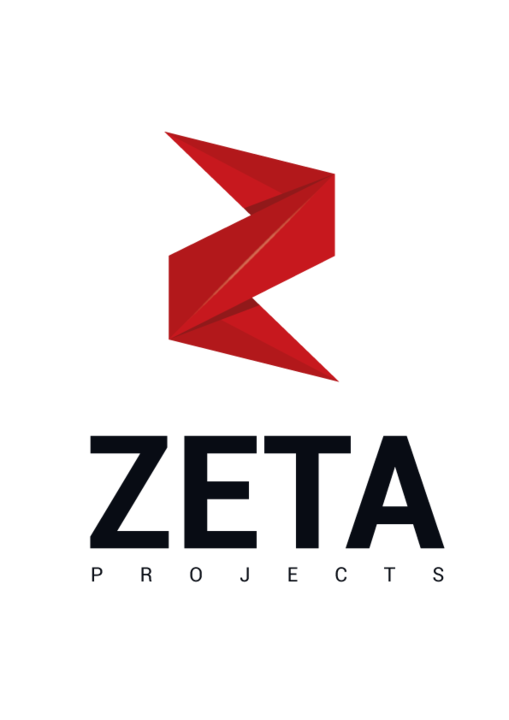
\includegraphics[width=3cm]{Images/Logo-ZetaProject.png}  & Ezzahra, Rue Habib Bourgiba    & Abrite les ingénieurs et les développeurs informatique  \\
	
	\hline
	
     \end{tabular}
     \caption{Les nouveaux locaux de Zeta Engineering en Tunisie}
     \label{1}
     \end{center}
     \label{tab1}
\end{table}

Notre projet consiste également à connecter les objets tels que les machines de pointage, le capteur de température et humidité, les lampes, les smartphones et les caméras de surveillance dans notre système d'information pour une utilisation plus efficace de ces ressources au sein de l'entreprise.

\subsection{Problématique}
La problématique de notre projet s'articule autour de trois domaines distincts, chacun présentant ses propres défis.

Le premier défi réside dans l'isolation des trois bureaux de ZETA, les empêchant de former un réseau local (LAN). Cette absence de connectivité entre les bureaux pose un obstacle majeur à la communication et au partage d'informations entre eux.

Deuxièmement, nous nous sommes confrontés à un problème lié à la gestion des informations. Il manque un système d'information centralisé pour nos applications IoT. Cela engendre des difficultés pour stocker, gérer et accéder aux données collectées par ces applications.

Enfin, l'intégration des dispositifs IoT constitue une autre problématique majeure. La plupart de ces appareils ne disposent pas d'une connectivité native pour rejoindre notre réseau ni pour interagir avec le système d'information que nous prévoyons de mettre en place.

Nous nous attacherons à résoudre ces problématiques tout au long de notre projet, en développant des solutions adaptées à chaque domaine, visant à améliorer la connectivité entre les bureaux, à établir un système d'information efficace, et à faciliter l'intégration des dispositifs IoT dans notre infrastructure.

\section{Méthodologie de travail et planification}

Dans cette section, nous abordons la présentation d'une méthodologie, ainsi que la problématique de notre projet.


\subsection{Présentation de la méthodologie en cascade}

Parmi les diverses méthodologies de gestion de projets telles que le modèle en V, les méthodologies itératives, Scrum, et bien d'autres, nous avons choisi d'adopter le modèle en cascade pour notre projet. Également connue sous le nom de méthodologie séquentielle, cette approche est souvent préférée dans les projets de Mémoire de Mastère en raison de sa simplicité et de sa facilité de compréhension.

Dans cette méthodologie, chaque étape doit être achevée avant que la suivante puisse commencer. Les étapes ne peuvent pas être rétrogradées et doivent être exécutées dans l'ordre établi. Cela signifie que le projet doit être entièrement défini et spécifié avant que la conception ne puisse commencer, et que la conception doit être terminée avant que la mise en œuvre puisse commencer, et ainsi de suite.


La figure \ref{Chap1.4} illustre les étapes caractéristiques de la méthodologie en cascade. Cette approche linéaire  et séquentielle guide le projet à travers une série d'étapes bien définies. Inities avec l'analyse des besoins et la planification, elle progresse ensuite vers la conception, la réalisation, les tests et enfin, la phase de déploiement et de maintenance. Chaque phase est traitée de manière séparée et successive, avec des étapes claires et spécifiques à accomplir avant de passer à la suivante. Cette structure rigoureuse garantit une progression ordonnée du projet, en mettant l'accent sur la finalisation de chaque étape avant de passer à la suivante.


\begin{figure}[H]
 \centering
    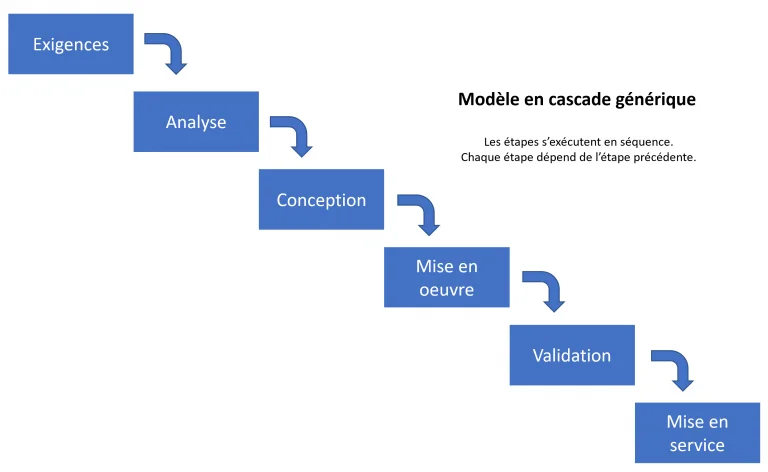
\includegraphics[width=15cm]{Images/cascade1.png}
    \caption{Méthodologie en Cascade \cite{blogcascade}}
    \label{Chap1.4}
\end{figure}

Le processus de la méthodologie en cascade se divise en plusieurs phases séquentielles, chacune étant une étape préalable à la suivante. Les étapes typiques incluent la définition des besoins, l'analyse, la conception, la mise en œuvre, les tests et la maintenance.



\subsection{Choix de la méthodologie en cascade}

Comme les besoins et les exigences du projet étaient relativement bien définis et stables dès le départ, le choix de la méthodologie en cascade s'est avéré approprié. Cette approche convient parfaitement lorsque les étapes du projet peuvent être planifiées à l'avance et que les changements ne sont pas fréquents.


De plus, notre équipe avait une compréhension claire des objectifs à atteindre et de la séquence des tâches à accomplir. La méthodologie en cascade nous a fourni un cadre structuré pour aborder chaque étape de manière méthodique, ce qui a permis une planification précise et une gestion efficace des ressources.



En résumé, chaque chapitre de notre rapport explique les choix matériels et logiciels adoptés, ainsi que la mise en œuvre de chaque composant du projet. Cette méthodologie nous permet de travailler de manière organisée et structurée, en veillant à ce que chaque étape soit achevée de manière adéquate avant de passer à la suivante \cite{fagarasan2021agile}.





\section{Conclusion }
En conclusion, ce premier chapitre nous a permis de présenter l'organisme d'accueil, Zeta Engineering, ainsi que le contexte du projet consistant à ouvrir trois nouveaux bureaux à Rades, Rades Meliane et Ezzahra.

Nous avons également abordé la méthodologie choisie pour la gestion de ce projet, à savoir la méthode en cascade, qui nous permet de travailler de manière séquentielle en terminant chaque phase avant de passer à la suivante. 

Les choix matériels et logiciels pour chaque étape sont également détaillés dans les chapitres suivants afin d'assurer une bonne exécution du projet.